%
% SchedWeekNight.tex
% Weekly Recurring Events Schedule, Night Shift
%
% Aleph Objects Operations Manual
%
% Copyright (C) 2014, 2015 Aleph Objects, Inc.
%
% This document is licensed under the Creative Commons Attribution 4.0
% International Public License (CC BY-SA 4.0) by Aleph Objects, Inc.
%

% Be sure to set the timestamp below, which prints the version number on the
% document, so it is easy to see if it is the latest version when printed out.

% These set the width of a day and the height of an hour.
\renewcommand*\daywidth{3.7cm}
\renewcommand*\hourheight{3.8em}

% The entry style will have two options:
% * the first option sets how many hours the entry will be (i.e. its height);
% * the second option sets how many overlapping entries there are (thus
%   determining the width).
\tikzset{entry/.style 2 args={
    xshift=(0.5334em+0.8pt)/2,
    draw,
    line width=0.8pt,
    font=\sffamily,
    rectangle,
    rounded corners,
    fill=blue!20,
    anchor=north west,
    inner sep=0.3333em,
    text width={\daywidth/#2-1.2em-1.6pt},
    minimum height=#1*\hourheight,
    align=center
}}

% Start the picture and set the x coordinate to correspond to days and the y
% coordinate to correspond to hours (y should point downwards).
\begin{sidewaysfigure}[p]
\thisfloatpagestyle{empty}
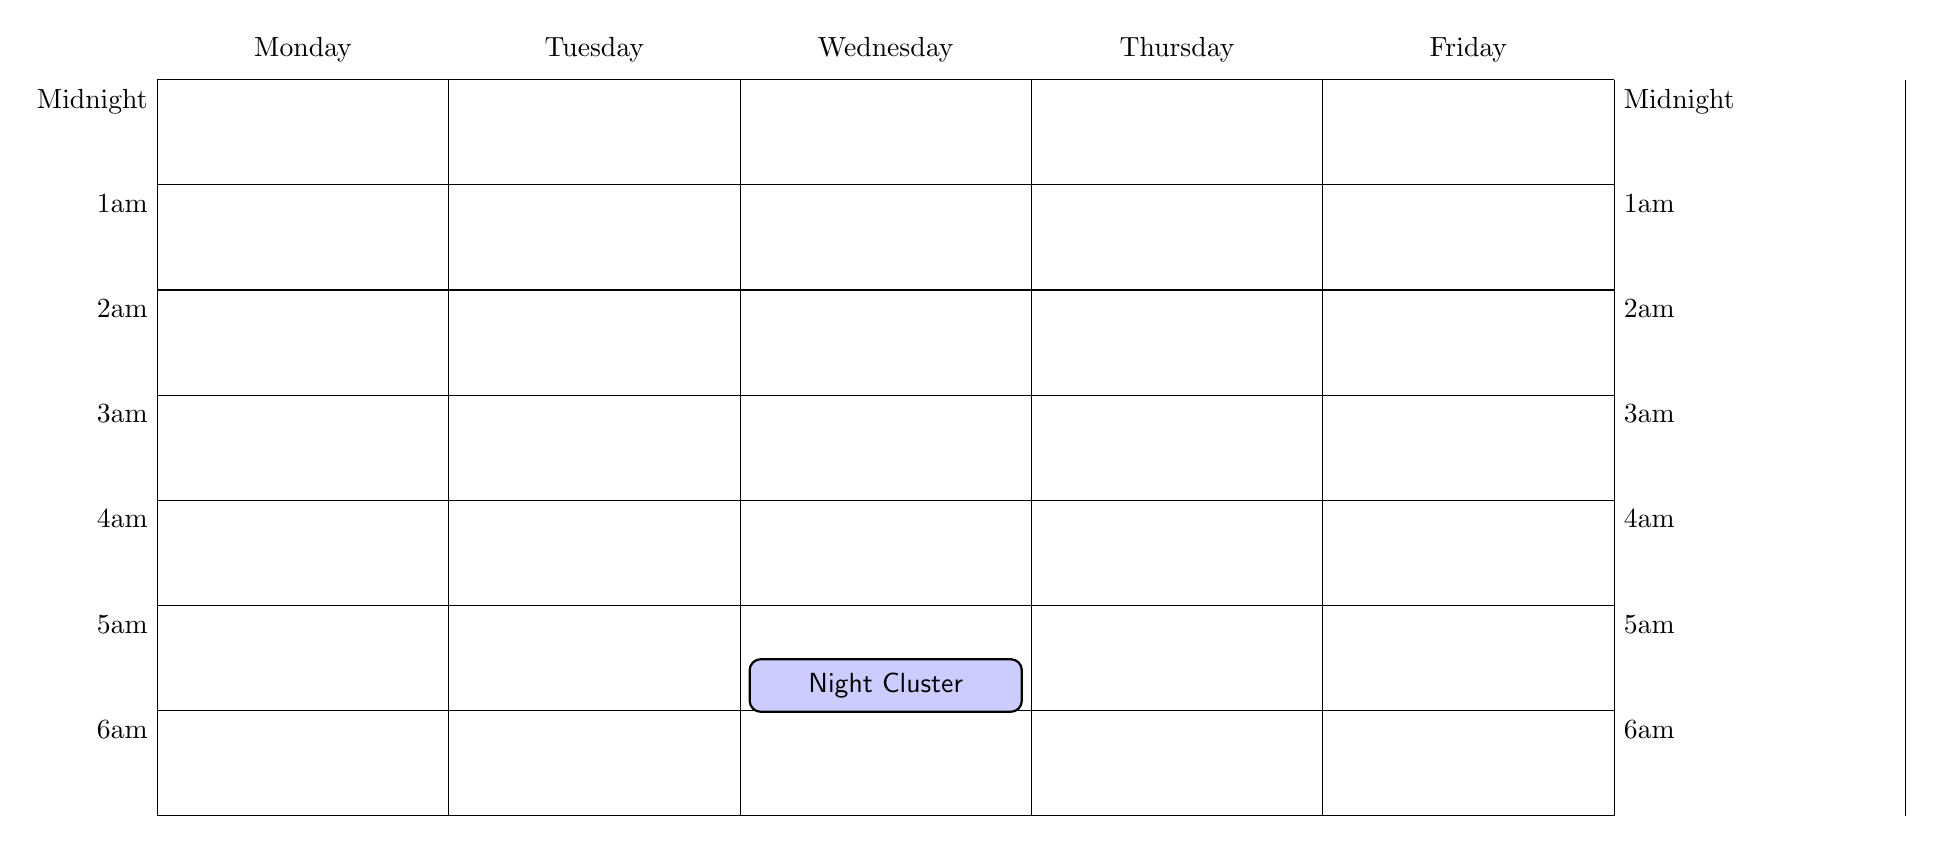
\begin{tikzpicture}[y=-\hourheight,x=\daywidth]

    % First print a list of times.
    \foreach \time/\ustime in {0/Midnight,1/1am,2/2am,3/3am,4/4am,5/5am,6/6am}
        \node[anchor=north east] at (1,\time) {\ustime};

    % Draw some day dividers.
    \draw (1,0) -- (1,7);
    \draw (2,0) -- (2,7);
    \draw (3,0) -- (3,7);
    \draw (4,0) -- (4,7);
    \draw (5,0) -- (5,7);
    \draw (6,0) -- (6,7);
    \draw (7,0) -- (7,7);
    
    % Draw some hour dividers.
    \draw (1,0) -- (6,0);
    \draw (1,1) -- (6,1);
    \draw (1,2) -- (6,2);
    \draw (1,3) -- (6,3);
    \draw (1,4) -- (6,4);
    \draw (1,5) -- (6,5);
    \draw (1,6) -- (6,6);
    \draw (1,7) -- (6,7);

    \foreach \time/\ustime in {0/Midnight,1/1am,2/2am,3/3am,4/4am,5/5am,6/6am}
        \node[anchor=north west] at (6,\time) {\ustime};
        
    % Start Monday.
    % Write the entries. Note that the x coordinate is 1 (for Monday) plus an
    % appropriate amount of shifting. The y coordinate is simply the starting
    % time.
    % 1=Monday, 2=Tuesday, 3=Wednesday, 4=Thursday, 5=Friday
    %\node[entry={DURATION}{COLUMN WIDTH?}] at (DAY,HOUR) {TEXT};

    % Monday
    \node[anchor=north] at (1.5,-0.5) {Monday};

    % Tuesday
    \node[anchor=north] at (2.5,-0.5) {Tuesday};
    
    % Wednesday
    \node[anchor=north] at (3.5,-0.5) {Wednesday};
    \node[entry={0.5}{1}] at (3,5.5) {Night Cluster};
    
    % Thursday
    \node[anchor=north] at (4.5,-0.5) {Thursday};
    
    % Friday
    \node[anchor=north] at (5.5,-0.5) {Friday};

\end{tikzpicture}
\caption{Weekly Company Meetings, Night Shift}
\renewcommand{\dateseparator}{}
% Timestamp Version: YYYY-MM-DD-Serial
\hfill\texttt{v.2015-07-07-1}

 \label{fig:ao_week_meet_night}
\end{sidewaysfigure}

